
\section{Two-term solution of the Boltzmann equation using BOLSIG+}

Electron impact involves the collision of an electron with (in this case neutral) atoms or molecules. If such an event takes place, this can lead to ionization, excited states and/or electron attachment processes. Also of interest are properties derived from an electron impact process such as the reduced electric field as a function of electron energy, and derived transport coefficients and reaction rates. To compute these properties it is necessary to first obtain the electron energy distribution function (EEDF), which under the conditions of a weakly-ionized plasma cannot be assumed to follow a Maxwellian distribution. To this end, the Boltzmann solver BOLSIG+ is used to obtain such distribution function and all derived transport and rate coefficients. This solver takes as input the cross-sections in $\rm m^2$ given as a function of the energy in eV and obtains the EEDF using a two-term approximation to this distribution.

\subsection{Settings: Physics}

The following parameters are selected in the BOLSIG+ interface:

\begin{itemize}
\item[1.]{AC field: NO}
\item[2.]{$E\times B$ field: NO}
\item[3.]{Superelastics: YES}
\item[4.]{electron-electron collisions: NO}
\item[5.]{electron-ion collisions: NO}
\item[6.]{Gas/excited states temperature: 300 K}
\end{itemize}
Changes to the latter 3 paramaters do not alter the results for $E/N$ vs electron temperature for the mixtures considered herein.

\subsection{Settings: Numerics}

The number of energy intervals is set to 200 with Automatic Grid type. All remaining convergence settings are kept to defaults.

\subsection{Settings: Advanced}

The following parameters are selected in the BOLSIG+ interface:

\begin{itemize}
\item[1.]{Include electron-neutral effects on Coulomb logarithm : YES}
\item[2.]{Ion charge parameter Z: 1.0}
\item[3.]{Ion-neutral mass ratio: 1.0}
\end{itemize}
All remaining parameters are kept to the default value.

\section{Reduced electric field vs electron temperature for various electron-neutral mixtures}

The electron energy range in which BOLSIG+ results are valid depend on the energy range of the corresponding cross-section data. Here, only the converged runs are kept, and any results extrapolated by BOLSIG+ are discarded. For higher electron temperatures for which there is no BOLSIG+ solution, the data is extrapolated by placing a spline control point for an electron temperature of $5\cdot10^6$ K, and a corresponding $E/N$ value that reflects the trend of the converged BOLSIG+ results. This last control point can be be modified to get the desired accuracy at very high temperatures. Results for several mixtures are shown below.

\subsection{Atomic hydrogen ($\rm H$)}

All the processes involving cross-sections used in the BOLSIG+ calculation are given in Table \ref{tab:tableH}. The reduced electric field results are shown in Fig. \ref{fig:electronimpact_4}.

\begin{table*}
  \center\fontsizetable
  \begin{threeparttable}
    \tablecaption{$\rm H$ electron impact processes with available cross-section data.}
    \label{tab:tableH}
    \fontsizetable
    \begin{tabular*}{\textwidth}{l@{\extracolsep{\fill}}llll}
    \toprule
    {no.}  & {process} & {type} &  {eV range}  &  {ref.} \\
    \midrule
      1 & $\rm e^- + H \rightarrow H^+ + e^- + e^-$  &  ionization   &  13.6-1000 &   \cite{lxc:2024:morgan} \\ 
      \midrule     
      2 & $\rm e^- + H \rightarrow e^- + H$  &  momentum transfer   &  0-1000  & \cite{lxc:2024:morgan}\\   
      \midrule
      3 & $\rm e^- + H \rightarrow e^- + H(2p) $  &  electronic excitation   &  10.2-1000 & \cite{lxc:2024:morgan}\\ 
      4 & $\rm e^- + H \rightarrow e^- + H(2s) $  &  electronic excitation   &  10.2-1000 & \cite{lxc:2024:morgan}\\ 
    \bottomrule
    \end{tabular*}
   \end{threeparttable}
\end{table*}

\begin{figure}[!ht]
\centering     %%% not \center
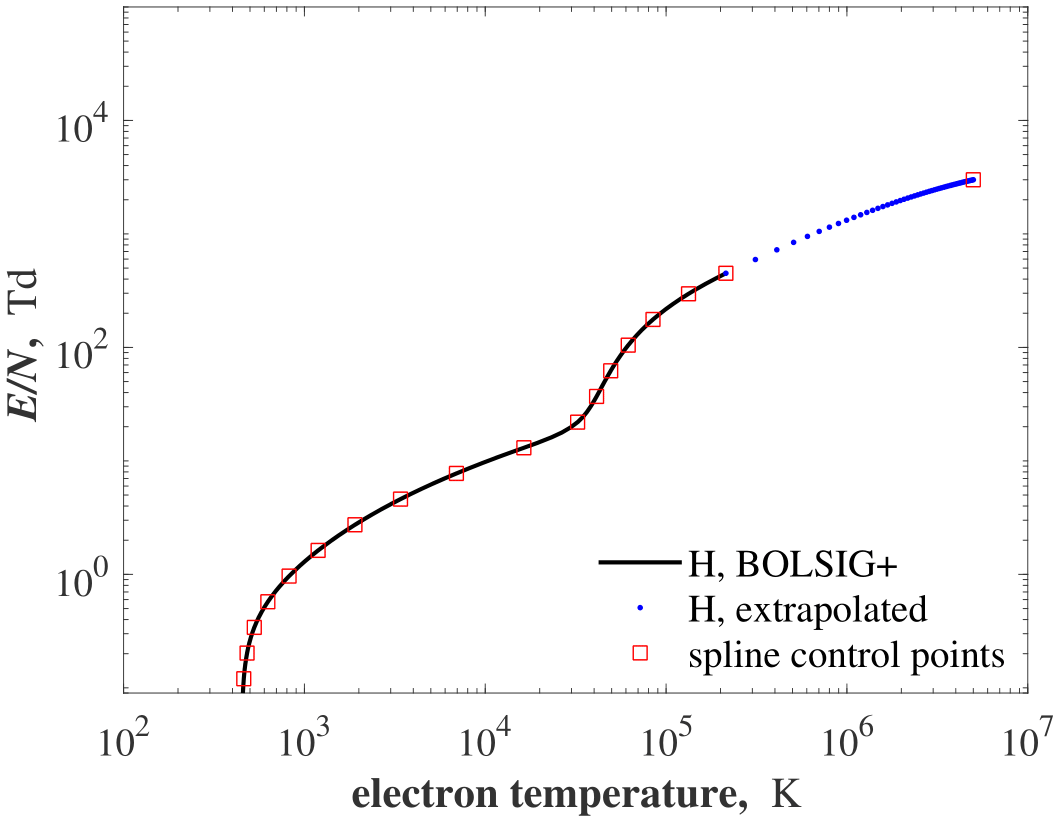
\includegraphics[width=0.7\linewidth, angle=0.0]{electronimpact_figs/electronimpact_fig4.png}
\caption{Reduced electric field as a function of the electron temperature for $\rm H$.}
\label{fig:electronimpact_4}
\end{figure}

\subsection{Atomic nitrogen ($\rm N$)}

\subsection{Atomic oxygen ($\rm O$)}

\subsection{Nitrogen molecule ($\rm N_2$)}

Experimental data for $E/N$ vs electron temperature is available from Ch.\ 21 of Ref.\ \citen{book:1997:grigoriev} for $\rm N_2$. In this case a cubic spline is fitted through the experimental data points and also through the remaining lower and upper ranges, if any, for which there is BOLSIG+ data. All the processes involving cross-sections used in the BOLSIG+ calculation are given in Table \ref{tab:tableN2}. The reduced electric field results are shown in Fig. \ref{fig:electronimpact_1}.

\begin{table*}
  \center\fontsizetable
  \begin{threeparttable}
    \tablecaption{$\rm N_2$ electron impact processes with available cross-section data.}
    \label{tab:tableN2}
    \fontsizetable
    \begin{tabular*}{\textwidth}{l@{\extracolsep{\fill}}llll}
    \toprule
    {no.}  & {process} & {type} &  {eV range}  &  {ref.} \\
    \midrule
      1 & $\rm e^- + N_2 \rightarrow N_2^+ + e^- + e^-$  &  ionization    &  15.6-1500 &   \cite{lxc:2024:morgan} \\ 
      \midrule     
      2 & $\rm e^- + NH_3 \rightarrow e^- + NH_3$  &  momentum transfer   &  0-1000  & \cite{lxc:2024:morgan}\\   
      \midrule
      3 & $\rm e^- + N_2 \rightarrow e^- + N_2^* $  &  rotational excitation   &  0.02-35 & \cite{lxc:2024:morgan}\\ 
           \midrule
      4 & $\rm e^- + N_2 \rightarrow e^- + N_2(V1)$  &  vibrational excitation   &  0.290-35 &\cite{lxc:2024:morgan}\\  
      5 & $\rm e^- + N_2 \rightarrow e^- + N_2(V1)$  &  vibrational excitation   &  0.291-35 &\cite{lxc:2024:morgan}\\  
      6 & $\rm e^- + N_2 \rightarrow e^- + N_2(V2)$  &  vibrational excitation   &  0.590-35 &\cite{lxc:2024:morgan}\\ 
      7 & $\rm e^- + N_2 \rightarrow e^- + N_2(V3)$  &  vibrational excitation   &  0.880-35 &\cite{lxc:2024:morgan}\\ 
      8 & $\rm e^- + N_2 \rightarrow e^- + N_2(V4)$  &  vibrational excitation   &  1.170-35 &\cite{lxc:2024:morgan}\\ 
      9 & $\rm e^- + N_2 \rightarrow e^- + N_2(V5)$  &  vibrational excitation   &  1.470-35 &\cite{lxc:2024:morgan}\\
      10 & $\rm e^- + N_2 \rightarrow e^- + N_2(V6)$  &  vibrational excitation   &  1.760-35 &\cite{lxc:2024:morgan}\\ 
      11 & $\rm e^- + N_2 \rightarrow e^- + N_2(V7)$  &  vibrational excitation   &  2.060-35 &\cite{lxc:2024:morgan}\\ 
      12 & $\rm e^- + N_2 \rightarrow e^- + N_2(V8)$  &  vibrational excitation   &  2.350-35 &\cite{lxc:2024:morgan}\\ 
          \midrule
      13 & $\rm e^- + N_2 \rightarrow e^- + N_2(A^3 \Sigma_{u}^+) $  &  electronic excitation   &  6.170-35 & \cite{lxc:2024:morgan}\\ 
      14 & $\rm e^- + N_2 \rightarrow e^- + N_2(A^3 \Sigma_{u}^+)$  &  electronic excitation   &  7.000-35 & \cite{lxc:2024:morgan}\\ 
      15 & $\rm e^- + N_2 \rightarrow e^- + N_2(B^3 \Pi_{g}) $  &  electronic excitation   &  7.350-35 & \cite{lxc:2024:morgan}\\ 
      16 & $\rm e^- + N_2 \rightarrow e^- + N_2(W^3 \Delta) $  &  electronic excitation   &  7.360-35 & \cite{lxc:2024:morgan}\\ 
      17 & $\rm e^- + N_2 \rightarrow e^- + N_2(A^3 \Sigma_{u}^+) $  &  electronic excitation   &  7.80-35 & \cite{lxc:2024:morgan}\\ 
      18 & $\rm e^- + N_2 \rightarrow e^- + N_2(B^3 \Sigma) $  &  electronic excitation   &  8.16-35 & \cite{lxc:2024:morgan}\\ 
      19 & $\rm e^- + N_2 \rightarrow e^- + N_2(A^1 \Sigma) $  &  electronic excitation   &  8.40-35 & \cite{lxc:2024:morgan}\\ 
      20 & $\rm e^- + N_2 \rightarrow e^- + N_2(A^1 \Pi) $  &  electronic excitation   &  8.55-35 & \cite{lxc:2024:morgan}\\ 
      21 & $\rm e^- + N_2 \rightarrow e^- + N_2(W^1 \Delta) $  &  electronic excitation   &  8.89-35 & \cite{lxc:2024:morgan}\\ 
      22 & $\rm e^- + N_2 \rightarrow e^- + N_2(C^3 \Pi) $  &  electronic excitation   &  11.03-35 & \cite{lxc:2024:morgan}\\ 
      23 & $\rm e^- + N_2 \rightarrow e^- + N_2(E^3 \Sigma) $  &  electronic excitation   &  11.88-35 & \cite{lxc:2024:morgan}\\  
      24 & $\rm e^- + N_2 \rightarrow e^- + N_2(A^1 \Sigma) $  &  electronic excitation   &  12.25-35 & \cite{lxc:2024:morgan}\\ 
      25 & $\rm e^- + N_2 \rightarrow e^- + N + N $  &  electronic excitation   &  13.00-35 & \cite{lxc:2024:morgan}\\ 
    \bottomrule
    \end{tabular*}
   \end{threeparttable}
\end{table*}

\begin{figure}[!ht]
\centering     %%% not \center
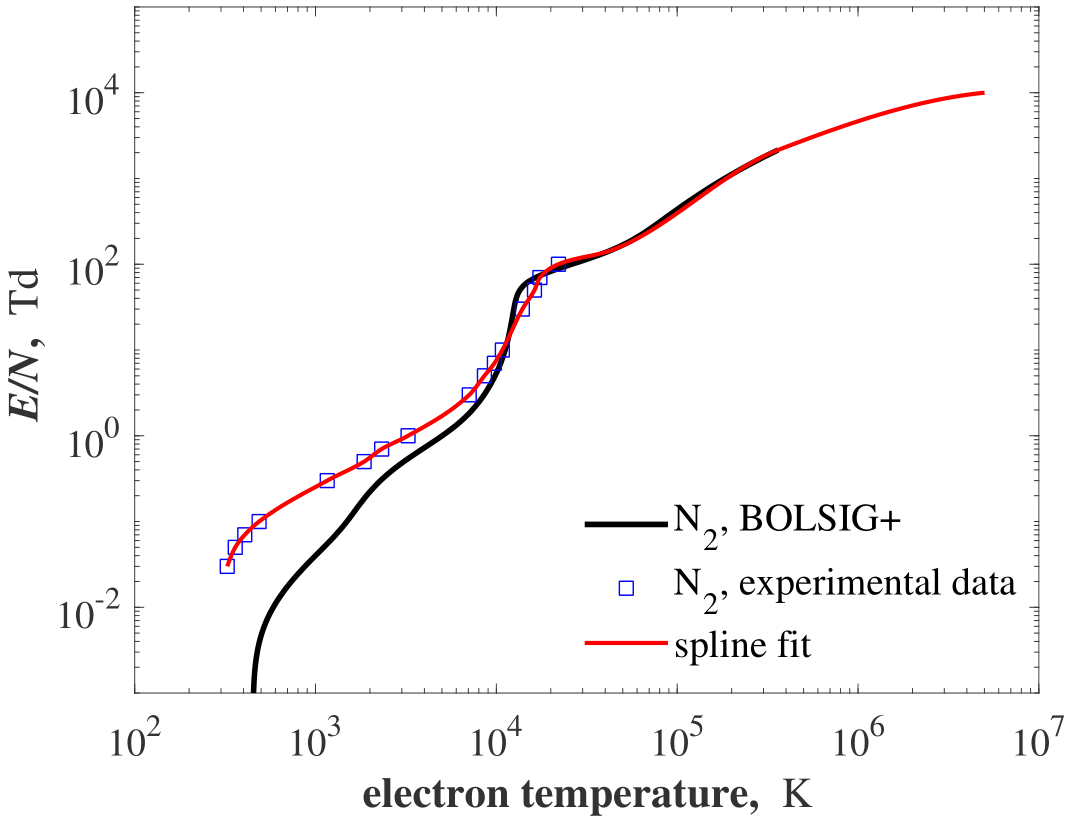
\includegraphics[width=0.7\linewidth, angle=0.0]{electronimpact_figs/electronimpact_fig1.png}
\caption{Reduced electric field as a function of the electron temperature for $\rm N_2$. Experimental data points are taken from \citen{book:1997:grigoriev}.}
\label{fig:electronimpact_1}
\end{figure}

\subsection{Oxygen molecule ($\rm O_2$)}

All the processes involving cross-sections used in the BOLSIG+ calculation are given in Table \ref{tab:tableO2}. Experimental data for $E/N$ vs electron temperature is available from Ch.\ 21 of Ref.\ \citen{book:1997:grigoriev} for $\rm O_2$. A cubic spline is fitted through the experimental data points and also through the remaining lower and upper ranges, if any, for which there is BOLSIG+ data.  The reduced electric field results are shown in Fig. \ref{fig:electronimpact_2}. In this case, no experimental data is available for $T_{\rm e}<1000$ K. Rather than make use of the BOLSIG+ results at low electron temperature which might not be accurate, we here prefer to extrapolate from the experimental data to lower $T_{\rm e}$. To do this, the experimental results for air are used and the corresponding $E/N$ value is obtained by summing the $\rm N_2$, $\rm O_2$ $E/N$ results weighed by their corresponding composition in dry air. The extrapolation of the $\rm O_2$ curve for $T_{\rm e}<1000$ K is such that there is good agreement between the experimental data and spline curve fit for air. The latter is shown in Fig. \ref{fig:electronimpact_5}.
%



\begin{table*}
  \center\fontsizetable
  \begin{threeparttable}
    \tablecaption{$\rm O_2$ electron impact processes with available cross-section data.}
    \label{tab:tableO2}
    \fontsizetable
    \begin{tabular*}{\textwidth}{l@{\extracolsep{\fill}}llll}
    \toprule
    {no.}  & {process} & {type} &  {eV range}  &  {ref.} \\
    \midrule
      1 & $\rm e^- + O_2 \rightarrow O_2^+ + e^- + e^-$  &  ionization   &  12.6-1500 &   \cite{lxc:2024:morgan} \\ 
      \midrule     
      2 & $\rm e^- + O_2 \rightarrow e^- + O_2$  &  momentum transfer   &  0-1000  & \cite{lxc:2024:morgan}\\   
      \midrule
      3 & $\rm e^- + O_2 \rightarrow e^- + O_2^* $  &  rotational excitation   &  0.38-20 & \cite{lxc:2024:morgan}\\ 
           \midrule
      4 & $\rm e^- + O_2 \rightarrow e^- + O_2(V1)$  &  vibrational excitation   &  0.57-15 &\cite{lxc:2024:morgan}\\  
      5 & $\rm e^- + O_2 \rightarrow e^- + O_2(V2)$  &  vibrational excitation   &  0.75-15 &\cite{lxc:2024:morgan}\\ 
          \midrule
      6 & $\rm e^- + O_2 \rightarrow e^- + O_2(A^1 \Delta) $  &  electronic excitation   &  0.977-45 & \cite{lxc:2024:morgan}\\ 
      7 & $\rm e^- + O_2 \rightarrow e^- + O_2(B^1 \Sigma) $  &  electronic excitation   &  1.627-45 & \cite{lxc:2024:morgan}\\ 
      8 & $\rm e^- + O_2 \rightarrow e^- + O_2(-) $  &  electronic excitation   &  4.50-45 & \cite{lxc:2024:morgan}\\ 
      9 & $\rm e^- + O_2 \rightarrow e^- + O_2(-) $  &  electronic excitation   &  6.00-45 & \cite{lxc:2024:morgan}\\ 
      10 & $\rm e^- + O_2 \rightarrow e^- + O_2(-) $  &  electronic excitation   &  8.40-45 & \cite{lxc:2024:morgan}\\ 
      11 & $\rm e^- + O_2 \rightarrow e^- + O_2(-) $  &  electronic excitation   &  9.97-100 & \cite{lxc:2024:morgan}\\ 
      12 & $\rm e^- + O_2 \rightarrow e^- + O + O $  &  electronic excitation   &  14.70-100 & \cite{lxc:2024:morgan}\\ 
    \bottomrule
    \end{tabular*}

   \end{threeparttable}
\end{table*}


\begin{figure}[!ht]
\centering     %%% not \center
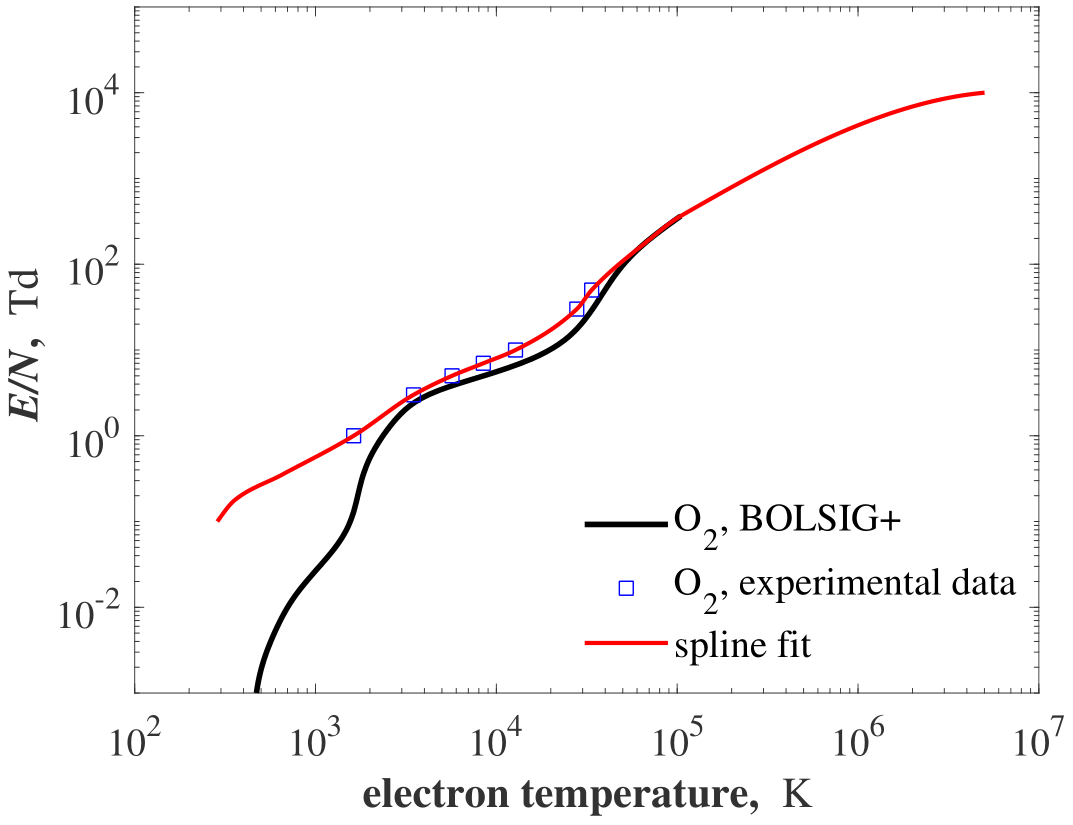
\includegraphics[width=0.7\linewidth, angle=0.0]{electronimpact_figs/electronimpact_fig2.png}
\caption{Reduced electric field as a function of the electron temperature for $\rm O_2$. Experimental data points are taken from \citen{book:1997:grigoriev}.}
\label{fig:electronimpact_2}
\end{figure}

\begin{figure}[!ht]
\centering     %%% not \center
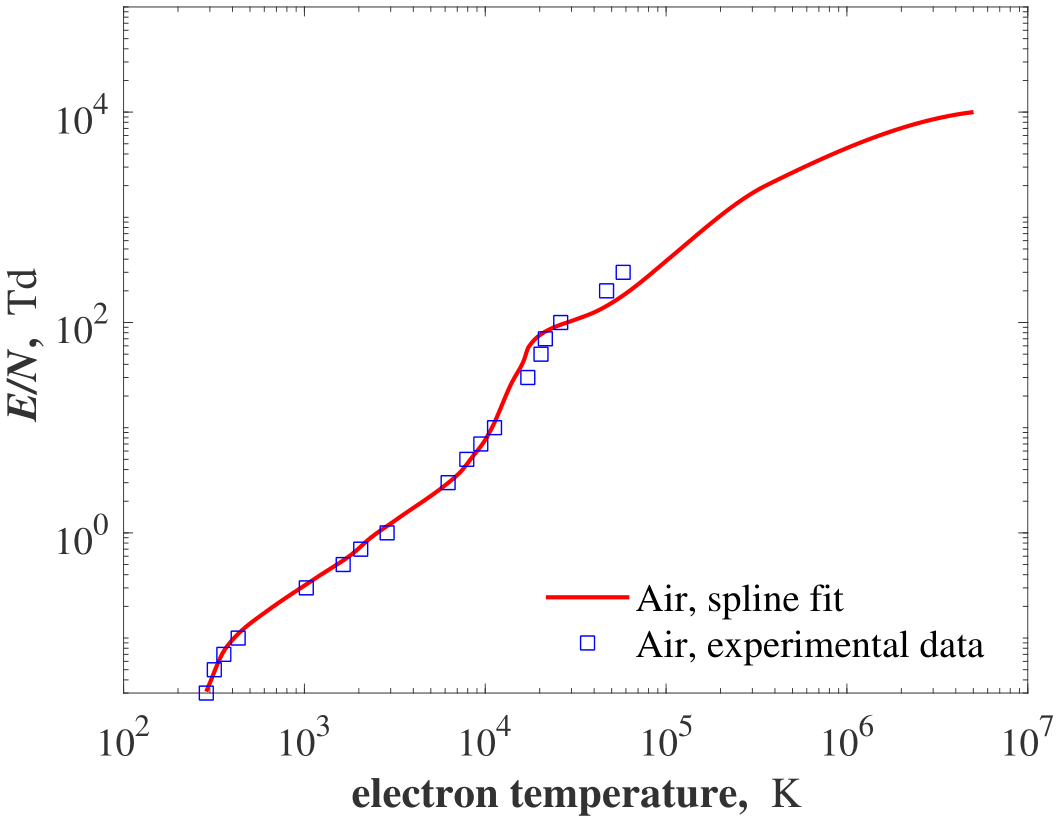
\includegraphics[width=0.7\linewidth, angle=0.0]{electronimpact_figs/electronimpact_fig5.png}
\caption{Reduced electric field as a function of the electron temperature for air. Experimental data points are taken from \citen{book:1997:grigoriev}.}
\label{fig:electronimpact_5}
\end{figure}

\subsection{Ammonia ($\rm NH_3$)}

All the processes involving cross-sections used in the BOLSIG+ calculation are given in Table \ref{tab:tableNH3}. The reduced electric field results are shown in Fig. \ref{fig:electronimpact_3}.


\begin{table*}
  \center\fontsizetable
  \begin{threeparttable}
    \tablecaption{$\rm NH_3$ electron impact processes with available cross-section data.}
    \label{tab:tableNH3}
    \fontsizetable
    \begin{tabular*}{\textwidth}{l@{\extracolsep{\fill}}llll}
    \toprule
    {no.}  & {process} & {type} &  {eV range}  &  {ref.} \\
    \midrule
      1 & $\rm e^- + NH_3 \rightarrow NH + H_2^+ + e^- + e^-$  &  ionization   &  10-1000 &  \cite{psst:2023:snoeckx} \\
      2 & $\rm e^- + NH_3 \rightarrow NH_3^+ + e^- + e^-$  &  ionization   &  10-1000  & \cite{psst:2023:snoeckx}\\
      3 & $\rm e^- + NH_3 \rightarrow NH_2 + H^+ + e^- + e^-$  &  ionization   &  20-1000   &\cite{psst:2023:snoeckx}\\
      4 & $\rm e^- + NH_3 \rightarrow NH_2^+ + H + e^- + e^-$  &  ionization   &  10-1000  & \cite{psst:2023:snoeckx}\\      
      5 & $\rm e^- + NH_3 \rightarrow N^+ + H_2 + H + e^- + e^-$  &  ionization   &  10-1000   &\cite{psst:2023:snoeckx}\\         
      6 & $\rm e^- + NH_3 \rightarrow NH^+ + H_2 +  e^- + e^-$  &  ionization   &  20-1000   &\cite{psst:2023:snoeckx}\\  
      \midrule     
      7 & $\rm e^- + NH_3 \rightarrow e^- + NH_3$  &  momentum transfer   &  0-4000  & \cite{lxc:2024:morgan}\\   
      \midrule
      8 & $\rm e^- + NH_3 \rightarrow e^- + NH_3(V2)$  &  electronic excitation   &  0.118-1000 & \cite{lxc:2024:morgan}\\ 
      9 & $\rm e^- + NH_3 \rightarrow e^- + NH_3(V4)$  &  electronic excitation   &  0.202-1000 &\cite{lxc:2024:morgan}\\  
      10 & $\rm e^- + NH_3 \rightarrow e^- + NH_3(V13)$  &  electronic excitation   &  0.420-1000 &\cite{lxc:2024:morgan}\\  
      11 & $\rm e^- + NH_3 \rightarrow e^- + NH_3(E1)$  &  electronic excitation   &  5.720-1000 &\cite{lxc:2024:morgan}\\ 
      12 & $\rm e^- + NH_3 \rightarrow e^- + NH_3(E2)$  &  electronic excitation   &  8.650-1000 &\cite{lxc:2024:morgan}\\ 
      \midrule
      13 & $\rm e^- + NH_3 \rightarrow e^- + NH_3(\nu_1)$  &  vibrational excitation   &  0.42-34 &\cite{psst:2023:snoeckx}\\  
      14 & $\rm e^- + NH_3 \rightarrow e^- + NH_3(\nu_2)$  &  vibrational excitation   &  0.12-32 &\cite{psst:2023:snoeckx}\\ 
      15 & $\rm e^- + NH_3 \rightarrow e^- + NH_3(\nu_3)$  &  vibrational excitation   &  0.45-35 &\cite{psst:2023:snoeckx}\\ 
      16 & $\rm e^- + NH_3 \rightarrow e^- + NH_3(\nu_4)$  &  vibrational excitation   &  0.21-35 &\cite{psst:2023:snoeckx}\\ 
      \midrule
      17 & $\rm e^- + NH_3 \rightarrow e^- + NH_3(00\rightarrow10)$  &  rotational excitation   &  0.01-30 & \cite{psst:2023:snoeckx}\\ 
      18 & $\rm e^- + NH_3 \rightarrow e^- + NH_3(00\rightarrow20)$  &  rotational excitation   &  0.01-30 &\cite{psst:2023:snoeckx}\\ 
      19 & $\rm e^- + NH_3 \rightarrow e^- + NH_3(00\rightarrow30)$  &  rotational excitation   &  0.01-30 &\cite{psst:2023:snoeckx}\\ 
      20 & $\rm e^- + NH_3 \rightarrow e^- + NH_3(00\rightarrow40)$  &  rotational excitation   &  0.01-30 &\cite{psst:2023:snoeckx}\\ 
      21 & $\rm e^- + NH_3 \rightarrow e^- + NH_3(00\rightarrow50)$  &  rotational excitation   &  0.01-30 &\cite{psst:2023:snoeckx}\\ 
    \bottomrule
    \end{tabular*}
   \end{threeparttable}
\end{table*}
%
\begin{figure}[!ht]
\centering     %%% not \center
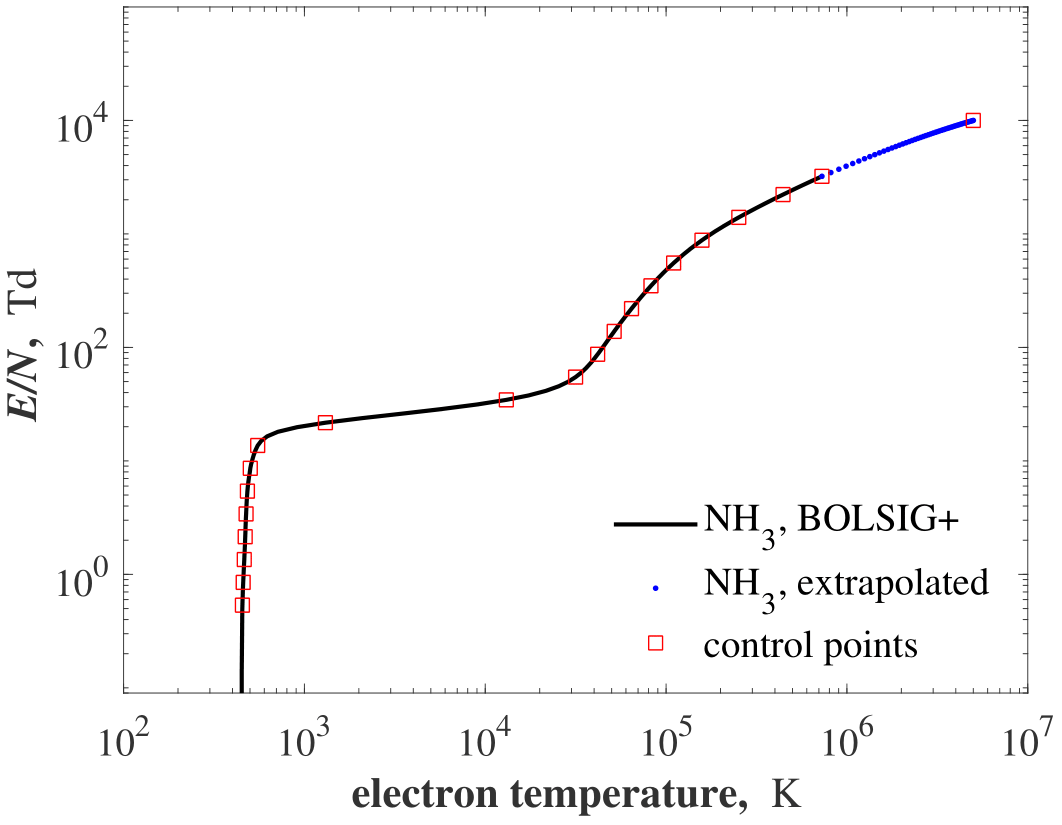
\includegraphics[width=0.7\linewidth, angle=0.0]{electronimpact_figs/electronimpact_fig3.png}
\caption{Reduced electric field as a function of the electron temperature for $\rm NH_3$.}
\label{fig:electronimpact_3}
\end{figure}




